%******************************************************************************%
%                                                                              %
%                                 Interlude                                    %
%                         for Machine Learning module                          %
%                                                                              %
%******************************************************************************%

% =============================== %
\section*{Interlude}
% =============================== %
\subsection*{Classification: The Art of Labelling Things}
% ******************************* %
Over the last three modules you have implemented your first machine learning algorithm.
You also discovered the three main steps we follow when we build \textbf{learning algorithms}:

\begin{figure}[!h]
    \centering
    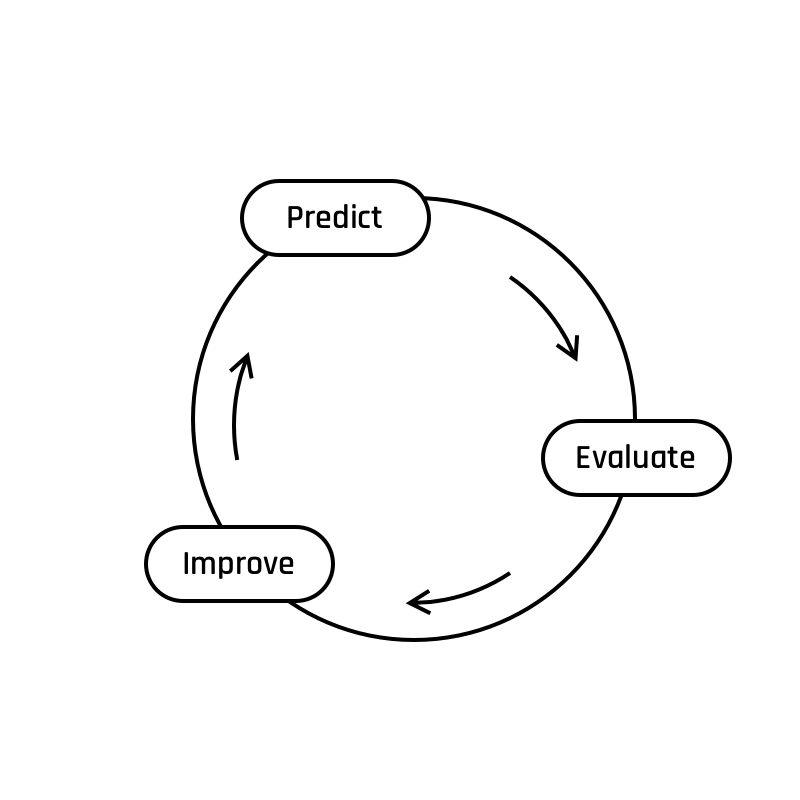
\includegraphics[scale=0.25]{assets/Default.png}
    %\caption{The Learning Cycle}
\end{figure}

The first algorithm you discovered, \textbf{Multivariate Linear Regression}, can now be used to predict a numerical value, based on several features.
This algorithm uses gradient descent to optimize its loss function.  

Now let's introduce you to your first \textbf{classification algorithm}: it is named \textbf{Logistic Regression.}
It peforms a \textit{classification task}, which means that you are not predicting a numerical value (like price, age, grades...) but \textbf{categories}, or \textbf{labels} (like dog, cat, sick/healty...).

\warn{
    Don't be confused by the word \textit{'regression'} in \textbf{Logistic Regression}.
    It really is a \textit{classification task}! The name is a bit tricky but you will quickly get used to it.
    \newline
    Once again: \textbf{Logistic Regression is a classification algorithm} which assigns a given example to a category.
}

\info{
    In this module we will use the following terms interchangeably: \textbf{class}, \textbf{category}, and \textbf{label}.
    They all refer to the \textit{groups} to which each training example can be assigned to, in a classification task.
}

% =============================== %
\subsection*{Predict I: Introducing the Sigmoid Function}
% ******************************* %

\begin{figure}[!h]
    \centering
    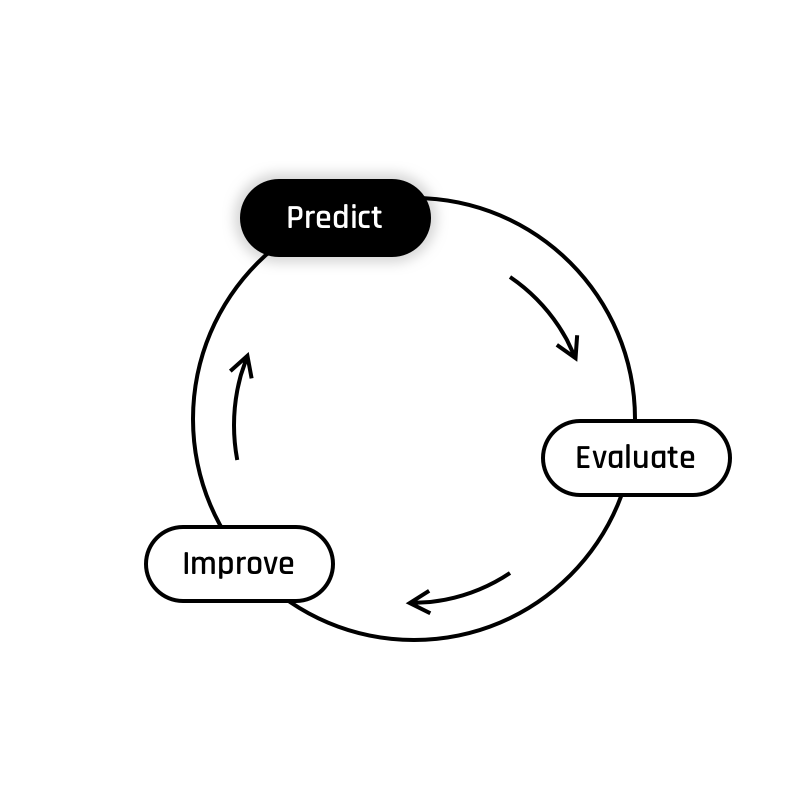
\includegraphics[scale=0.25]{assets/Predict.png}
    %\caption{The Learning Cycle - Predict}
\end{figure}

% =============================== %
\subsubsection*{Formulating a Hypothesis}
% ******************************* %
Remember that a hypothesis, denoted $h(\theta)$, is an equation that combines a set of \textbf{features} (that characterize an example) with \textbf{parameters} in order to output a \textbf{prediction}.
Remember the hypothesis we used in linear regression?  

$$
h(\theta) = \theta_0 + \theta_{1} x_{1}^{(i)} + \dots + \theta_{n} x_{n}^{(i)} = \theta \cdot x'^{(i)}
$$

It worked fine to predict continuous values, but could we also use it to tell, for example, if a patient is sick or not?
That's a yes-or-no question, so the output from the hypothesis function should reflect that.

To get started, we'll assign each class a numerical value: sick patients will be assigned a value of 1, and healthy patients will be assigned a value of 0.
The goal will be to build a hypothesis that outputs a probability that a patient is sick, as a float number within the range of 0 and 1.

The good news is that we can keep the linear equation we already worked with!
All we need to do is squash its output through another function that is bounded between 0 and 1.
That's the \textbf{Sigmoid function} and your next exercise is to implement it!
